\documentclass{article}
\usepackage{amsmath}
\usepackage[utf8]{inputenc}
\usepackage{graphicx}
\usepackage{verbatim}
\usepackage{float}
\usepackage[makeroom]{cancel}
\usepackage[english]{babel}
\usepackage{textcomp}
\usepackage{gensymb}
\usepackage{color}
\usepackage{subcaption}
\usepackage{caption}
\usepackage{hyperref}
\usepackage{physics}
\usepackage{dsfont}
%\usepackage{amsfonts}
\usepackage{listings}
\usepackage{multicol}
\usepackage{units}

% From Eirik's .tex
\usepackage{epstopdf}
\usepackage{cite}
\usepackage{braket}
\usepackage{url}
\bibliographystyle{plain}

\usepackage{algorithmicx}
\usepackage{algorithm}% http://ctan.org/pkg/algorithms
\usepackage{algpseudocode}% http://ctan.org/pkg/algorithmicx

\usepackage[margin=1cm]{caption}
\usepackage[outer=1.2in,inner=1.2in]{geometry}
% For writing full-size pages
%\usepackage{geometry}
%\geometry{
%  left=5mm,
%  right=5mm,
%  top=5mm,
%  bottom=5mm,
%  heightrounded,
%}

% Finding overfull \hbox
\overfullrule=2cm

\lstset{language=IDL}
 %\lstset{alsolanguage=c++}
\lstset{basicstyle=\ttfamily\small}
 %\lstset{backgroundcolor=\color{white}}
\lstset{frame=single}
\lstset{stringstyle=\ttfamily}
\lstset{keywordstyle=\color{red}\bfseries}
\lstset{commentstyle=\itshape\color{blue}}
\lstset{showspaces=false}
\lstset{showstringspaces=false}
\lstset{showtabs=false}
\lstset{breaklines}
\lstset{aboveskip=20pt,belowskip=20pt}

\lstset{basicstyle=\footnotesize, basewidth=0.5em}
\lstdefinestyle{cl}{frame=none,basicstyle=\ttfamily\small}
\lstdefinestyle{pr}{frame=single,basicstyle=\ttfamily\small}
\lstdefinestyle{prt}{frame=none,basicstyle=\ttfamily\small}
% \lstinputlisting[language=Python]{filename}


\definecolor{codepurple}{rgb}{0.58,0,0.82}
\definecolor{backcolour}{rgb}{0.95,0.95,0.92}
\definecolor{dkgreen}{rgb}{0,0.6,0}
\definecolor{gray}{rgb}{0.5,0.5,0.5}
\definecolor{magenta}{rgb}{0.58,0,0.82}

\lstdefinestyle{pystyle}{
  language=Python,
  aboveskip=3mm,
  belowskip=3mm,
  columns=flexible,
  basicstyle={\small\ttfamily},
  backgroundcolor=\color{backcolour},
  commentstyle=\color{dkgreen},
  keywordstyle=\color{magenta},
  numberstyle=\tiny\color{gray},
  stringstyle=\color{codepurple},
  basicstyle=\footnotesize,
  breakatwhitespace=false,
  breaklines=true,
  captionpos=b,
  keepspaces=true,
  numbers=left,
  numbersep=5pt,
  showspaces=false,
  showstringspaces=false,
  showtabs=false,
  tabsize=2
}

%%%%%%%%%%%%%%%%%%%%%%%%%%%%%%%%
% Self made macros here yaaaaaay
\newcommand\answer[1]{\underline{\underline{#1}}}
\newcommand\pd[2]{\frac{\partial #1}{\partial #2}}
\newcommand\red[1]{\textcolor{red}{\textbf{#1}}}
\newcommand\numberthis{\addtocounter{equation}{1}\tag{\theequation}}
% Usage: \numberthis \label{name}
% Referencing: \eqref{name}

% Some matrices
\newcommand\smat[1]{\big(\begin{smallmatrix}#1\end{smallmatrix}\big)}
\newcommand\ppmat[1]{\begin{pmatrix}#1\end{pmatrix}}

% Section labeling
\usepackage{titlesec}% http://ctan.org/pkg/titlesec
\renewcommand{\thesubsection}{\arabic{subsection}}


% Title/name/date
\title{FYS4150 - Project 2}
\author{Simen Nyhus Bastnes \& Eirik Ramsli Hauge}
\date{3. October 2016}

\begin{document}
\maketitle

\begin{abstract}
Wow dude, so this is like, so abstract dude. Have you ever had a dream that you, um, you had, your, you- you could, you’ll do, you- you wants, you, you could do so, you- you’ll do, you could- you, you want, you want them to do you so much you could do anything?
\end{abstract}
\subsection{Introduction}
In project 2, we aim to solve Schrödinger's equation for two electrons with and without a repulsive Coulomb interaction in a three-dimensional harmonic oscillator well. We start by reformulating the equation in a discretized form as an eigenvalue equation, which can be solved with Jacobi's method. \\\\We can then compare our implementation Jacobi's method fares against ``smarter'' algorithms for solving eigenvalue equations. Finally, we will look at implementing unit-tests, in order to test that the various parts of our program does what it's intended to do.\\\\
\red{Should maybe be rewritten, or changed order, or add more, dunno}
\subsection{Theory}
\subsubsection{Schrödinger's equation}
In this project, we will assume that the electrons move in a three-dimensional harmonic oscillator potential, and repel each other via the static Coulomb interaction. By assuming spherical symmetry, the solution for the radial part of Schrödinger's equation for one electron reads
\begin{align*}
  -\frac{\hbar^2}{2m}\bigg(\frac{1}{r^2}\frac{d}{dr}r^2\frac{d}{dr} - \frac{l(l+1)}{r^2}\bigg)R(r) + V(r)R(r) = ER(r)\numberthis\label{eq:radial_schroedinger}
\end{align*}
For the rest of the project, we set the orbital momentum quantum number $l$ to zero. In our non-interacting case, the harmonic oscillator potential $V(r) = (1/2)kr^2$ with $k=m\omega^2$.\\\\We perform a substitution for $R(r) = (1/r)u(r)$, introduce a dimensionless variable $\rho = (1/\alpha)r$, where $\alpha$ is a constant with dimension length $\alpha = (\hbar^2/mk)^{1/4}$. Inserting this into the Scrödinger equation \eqref{eq:radial_schroedinger}, we get
\begin{align*}
-\frac{d^2}{d\rho^2}u(\rho) + \rho^2u(\rho) = \lambda u(\rho)\numberthis\label{eq:dimless_schroedinger}
\end{align*}
where $\lambda = (2m\alpha^2/\hbar^2)E$. Equation \eqref{eq:dimless_schroedinger} is the first equation we want to solve numerically, and we will later use that for $l=0$, the first eigenvalues $\lambda$ are $\lambda_0 = 3$, $\lambda_1 = 7$ and $\lambda_2 = 11$.\\\\
Starting our journey to write equation \eqref{eq:dimless_schroedinger} as an eigenvalue equation, we use the by now standard expression for the second derivative
\begin{align*}
  u'' = \frac{u(\rho+h)-2u(\rho)+u(\rho-h)}{h^2}+\mathcal{O}(h^2)
\end{align*}
where $h$ is our step length. We define minimum and maximum values for $\rho$, $\rho_{\text{min}} = 0$ and $\rho_{\text{max}}$, as we cannot set $\rho_{\text{max}} = \infty$. Next, we split this interval into $N$ number of mesh points, so that we can define the step length as
\begin{align*}
  h = \frac{\rho_N-\rho_0}{N}
\end{align*}
where $\rho_0 = \rho_{\text{min}}$ and $\rho_{\text{max}} =\rho_N$. This gives us an expression for $\rho$ at point $i$
\begin{align*}
  \rho_i = \rho_0 + ih\;\;\;\;\;\;\;\;\;i=1,2,\dots,N
\end{align*}
Now we can rewrite the second derivative as
\begin{align*}
  u_i'' = \frac{u_{i+1}-2u_i + u_{i-1}}{h^2}
\end{align*}
Using this, we can rewrite the dimensionless Schrödinger equation \eqref{eq:dimless_schroedinger} as a discretized equation.
\begin{align*}
  -\frac{u_{i+1}-2u_i+u_{i-1}}{h^2} + \rho_i^2u_i = -\frac{u_{i+1}-2u_i+u_{i-1}}{h^2} + V_iu_i = \lambda u_i 
\end{align*}
where $V_i = \rho_i^2$ is the harmonic oscillator potential. We can represent the left-hand side as a matrix multiplied by a vector $u$
\subsubsection*{Interacting case}
\begin{align*}
  V(\rho) = \omega_r^2\rho^2 + 1/\rho
\end{align*}
\subsubsection{Jacobi's method}
\subsection{Experimental?}
\subsection{Results}
\subsection{Discussion}
\begin{figure}[H]
  \centering
  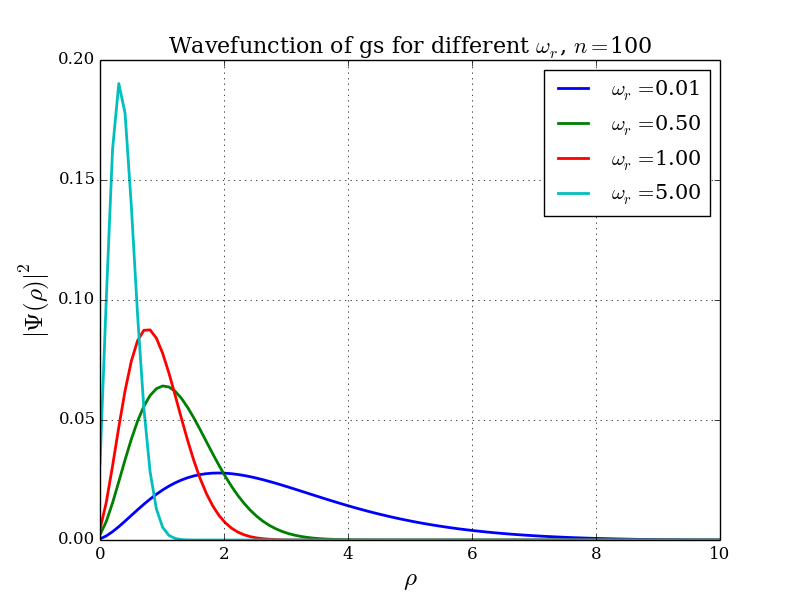
\includegraphics[scale=0.5]{../figures/eigvec_interact_n100.png}
  \caption{Plot of the eigenvectors for the interacting case for $n=100$}
  \label{fig:eigvec100}
\end{figure}
\subsection{Conclusion}
\bibliography{references}
\end{document}
